\[ \zeta(z) - \frac1{z-1} = \underbrace{\frac1{\Gamma(z+n)}}_{\footnotemark}\footnotetext{{holomorphic in $\C$ (with zeros at $-n$, $-n-1$, $\dotsc$)}} \underbrace{\int_0^\infty t^{z+n-1} g^{(n)}(t)\d t}_{\footnotemark}\footnotetext{{holomorphic for $\Re(z)>-n$}} \]
We can see that $\zeta(z)-\frac1{z-1}$ can be extended to be holomorphic for $\Re(z)>-n$. \\
\xout{Also, we can see that $\zeta(z)$ has zeros at $0$, $-1$, $-2$, $\dotsc$.} \\
In fact $\zeta(z)$ has zeros at $z=-2$, $-4$, $-6$, $\dotsc$.

Riemann Xi function
\[ \xi(z) = \frac{z(z-1)\Gamma(\frac z2)}{2\pi^{z/2}}\zeta(z) ? \]
This is entire with $\xi(z)=\xi(1-z)$.

\thm (Landau's Convergence Theorem) \\
Let $\sum\frac{f(n)}{n^z}$ be a Dirichlet series with real non-negative coefficients $f(n)\geq0$ and with finite abscissa $\sigma_c$.  Then $F(z)=\sum_{n=1}^\infty\frac{f(n)}{n^z}$ is singular at $\sigma_c$. \\
\pf Suppose for a contradiction, that $F(z)$ can be extended to be holomorphic in $D(\sigma_c,r)$.  Let $a=1+\sigma_c$.
\[ 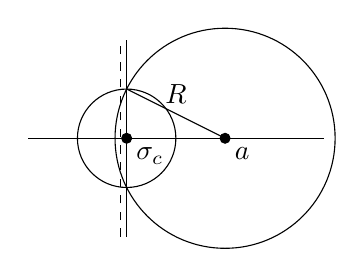
\begin{tikzpicture}[scale=1.25]
\draw(-1,0)--(2,0);
\draw(0,-1)--(0,1);
\draw[fill](0,0)circle(0.05);
\draw[fill](1,0)circle(0.05);
\draw(0,0)circle(0.5);
\draw(1,0)circle({sqrt(5/4)});
\node[below right]at(0,0){$\sigma_c$};
\node[below right]at(1,0){$a$};
\draw(1,0)--(0,0.5)node[above,midway]{$R$};
\draw[dashed]({(1-sqrt(5/4))/2},-1)--({(1-sqrt(5/4))/2},1);
\end{tikzpicture} \]
Choose $R>0$ so that $F(z)$ is holomorphic in $D(a,R)$ and $R>a-\sigma_c$.
For $z$ with $\Re(z)>\sigma_c$
\begin{align*}
F(z) &= \sum_{n=1}^\infty \frac{f(n)}{n^z} \\
F'(z) &= \sum_{n=1}^\infty \frac{-(\log n)f(n)}{n^z} \\
&\eqvdots \\
F^{(k)}(z) &= \sum_{n=1}^\infty \frac{(-1)^k (\log n)^k f(n)}{n^z}
\end{align*}
For $z\in D(a,R)$ we have
\begin{align*}
F(z) &= \sum_{k=0}^\infty \frac{F^{(k)}(a)}{k!} (z-a)^k \\
&= \sum_{k=0}^\infty \underbrace{\sum_{n=1}^\infty \frac{(-1)^k (\log n)^k f(n)}{k!n^a}}_{\text{converges}} (z-a)^k
\end{align*}
\aside
\begin{align*}
F(z) &= \sum \frac{f(n)}{n^z} = \frac{f(n)}{n^{z-a}\cdot n^a}\footnote{$\frac1{n^{z-a}}=e^{-(z-a)\log n}$} \\
&= \sum_{n=1}^\infty \frac{f(n)}{n^a}e^{(a-z)\log n} \\
&= \sum_{n=1}^\infty \frac{f(n)}{n^a} \sum_{k=0}^\infty \frac{(\log n)^k}{k!} (a-z)^k
\end{align*}
In particular, this converges for some values $z\in\R$ with $z<\sigma_c$.
Then all the terms in the series
\[ \sum_{k=0}^\infty \sum_{n=1}^\infty \frac{(\log n)^kf(n)}{k!n^a} (a-z)^k \]
are non-negative
so we can interchange summation to get
\[ F(z) = \sum_{n=1}^\infty \sum_{k=0}^\infty \frac{(\log n)^k f(n)}{k!n^a} (a-z)^k = \dotsb = \sum_{n=1}^\infty \frac{f(n)}{n^z} . \]
Thus the original Dirichlet series converges for some $z\in\R$ with $z<\sigma_c$, and this is not possible.

\thm $\zeta(z)\neq0$ for $\Re(z)\geq1$. \\
\pf We already know that $\zeta(z)\neq0$ for $\Re(z)>1$ (since for $\Re(z)>1$ we have
\[ \zeta(z) = \sum_{n=1}^\infty \frac1{n^z} \co M(z) = \sum_{n=1}^\infty \frac{\mu(n)}{n^z} \]
and
\[ \zeta(z)\cdot M(z) = \sum_{k,l} \frac{1}{k^z}\cdot\frac{\mu(l)}{l^z} = \sum_{n=1}^\infty \frac{1}{n^z} \sum_{d\div n} \mu(d) = 1 \]
so $\zeta(z)\neq0$ for $\Re(z)>1$.)\footnote{$\zeta(z)=\prod_p\frac{1}{1-p^{-z}}$, $M(z)=\prod_p(1-p^{-z})$} \\
It remains to show that $\zeta(z)\neq0$ for $\Re(z)=1$.

Suppose, for a contradiction, $\zeta(1+ia)=0$ where $0\neq a\in\R$.
Since $\zeta(\overline{z})=\overline{\zeta(z)}$ we also have $\zeta(1-ia)=0$.

Note that the function $\zeta(z)\zeta(z+ia)$ is holomorphic in all of $\C$ since the zero of $\zeta(z+ia)$ cancels the pole of $\zeta(z)$ at $z=1$ and the zero of $\zeta(z)$ cancels the pole of $\zeta(z+ia)$ at $z=1-ia$.

Similarly $\zeta(z)\zeta(z-ia)$ is holomorphic in $\C$.
Let $F(z)=\zeta(z)^2\zeta(z+ia)\zeta(z-ia)$ which is holomorphic in $\C$.
We calculate the coefficients for the Dirichlet series of $F(z)$.
For $\Re(z)>1$
\begin{align*}
F(z) &= \zeta(z)^2 \zeta(z+ia) \zeta(z-ia) \\
&= \prod_p \paren[\Big]{\frac{1}{1-p^{-z}}}^2 \prod_p \paren[\Big]{\frac{1}{1-p^{-z-ia}}} \prod_p \paren[\Big]{\frac{1}{1-p^{-z+ia}}} .
\end{align*}
Using the principal branch of the logarithm on the right, and some branch on the left\footnote{Aside:
\[ \frac{1}{1-x} = 1 + x + x^2 + \dotsb \qquad\qquad -\log(1-x) = x + \frac12 x^2 + \frac13 x^3 + \dotsb \]}
\begin{align*}
\log F(z) &= - \sum_p 2 \log(1-p^{-z}) + \log(1-p^{-z-ia}) + \log(1-p^{-z+ia}) \\
&= \sum_p \sum_{k=1}^\infty \paren[\Big]{ \frac{2}{kp^{kz}} + \frac{1}{kp^{kz+ika}} + \frac{1}{kp^{kz-ika}} } \\
&= \sum_p \sum_{k\geq1} \frac{1}{kp^{kz}} \paren[\Big]{ 2 + p^{-ika} + p^{ika} } \\
&= \sum_p \sum_{k\geq1} \frac{2}{kp^{kz}} \paren{ 1 + \cos(ka\log p) }\footnote{Aside:
\[ p^{-ika}+p^{ika} = e^{-ika\log p}+e^{ika\log p}=2\cos(ka\log p) \]
for $n=p^k$, $\log n=k\log p=k\Lambda(n)$, $\frac1k=\frac{\Lambda(n)}{\log n}$} \\
&= \sum_{n=p^k} \frac{2\Lambda(n)(1+\cos(a\log n))}{\log n\cdot n^z} \\
&= \sum_n \frac{g(n)}{n^z} \\ \intertext{where $g(n)=\frac{2\Lambda(n)(1+\cos(a\log n))}{\log n}$}
\therefore F(z) &= e^{\sum_{n=1}^\infty\frac{g(n)}{n^z}} = \sum_{k=0}^\infty \frac{1}{k!}\paren[\Big]{\sum_{n=1}^\infty\frac{g(n)}{n^z}}^k
\end{align*}
If we expand this, we will find that the coefficients of $F(z)$ are real and non-negative.
\[ F(z) = \zeta(z)^2 \zeta(z+ia) \zeta(z-ia) \]
is holomorphic in $\C$ and $F(z)=\sum_{n=1}^\infty\frac{f(n)}{n^z}$ with each $f(n)\geq0$ so by Landau's Theorem $\sigma_c$ is not finite so $\sigma_c=-\infty$ so $\sum\frac{f(n)}{n^z}$ converges absolutely for all $z\in\C$.
